\chapter{Artefact Design} \label{a-d}

\section{Introduction} \label{a-d--introduction}

In Chapter 2 we identified that blah blah...
This chapter describes the design of blah blah, a system that blah blah.  First, the chapter describes the project’s design methodology (section 3.2), and system requirements (section 3.3).  A proposed solution is then discussed (section 3.4), followed by a blah blah....


\section{Design Methodology} \label{a-d--methodology}

The design and development of blah blah

\subsection{A Review of Existing Software} \label{a-d--review-of-existing-software}

This section is a review of current home-brewing software.

\subsubsection{BeerSmith}

+ Cross platform (Macintosh, Ubuntu and Windows)

\subsubsection{BeerTools Pro}
\subsubsection{Beer Calculus}
\subsubsection{ProMash}
\subsubsection{BrewPal}
\subsubsection{BrewTarget}
\subsubsection{BeerAlchemy}
\subsubsection{Brewer's Friend}

% Need to review the rest of the brewing software https://homebrew.stackexchange.com/questions/784/what-software-do-most-brewers-use/898]

One thing that is common among all of these choices is their inherent offline nature. As they are installed directly to the computer and not in a web browser.

\subsection{Software Life-cycle Methodology} \label{a-d--methodology--life-cycle}

Choosing a methodology is never one size fits all. Instead considering the environment and team around a project is important. Agile software development offers principles that work well with a team, however there is a lot that can be taken for any project.

Agile development embraces changes in development life-cycle and adapts to them, this is in contrast to traditional plan-driven development in which predictions are used instead. An agile plan is the initial set of goals which will adapt as the project grows. \cite{fowler_agile}

Using an incremental and evolutionary approach is key for this artefact due to it's experimental nature, the goals and proposed solutions will change through-out development.

\subsection{Tools and Services} \label{a-d--methodology--tools}

Kanban boards are a tool to visualise the workflow for a project, an online implementation of this tool is Trello. Trello can be used for multiple scenarios and fits well for a software project. Features, bugs and other research can be represented by cards. \cite{trello} % cite for kanban

Version control is arguably one of the most important tools in software development. It records changes over time so that a previous version of the project can be revisited later. Git is a free and open source distributed version control system that is used on many projects. \cite{git}

While being distributed it's often useful to have a centralized repository, there are many Git repository hosting services. GitHub and Bitbucket are two popular choices. While GitHub encourages Open Source Software on their platform the service itself isn't Open Source. \cite{github} GitLab started as a GitHub clone that is fully Open Source, with the choice to host yourself or use their servers. \cite{gitlab} \cite{bitbucket}

These platforms offer similar features but the artefact will be hosted with GitHub due to the familiarity to the author and also the features it offers.

GitHub has a system of `Issues', which allow for tasks to be tracked. These issues can be commented and then closed when deemed completed. For this project the following labels are used:

\begin{itemize}
  \item \textbf{\colorbox{red}{bug}} - tasks which define a bug in the project
  \item \textbf{\colorbox{blue}{feature}} -  tasks which introduce a new feature to the project
  \item \textbf{\colorbox{yellow}{report}} - tasks which are relevant to the report writing itself
  \item \textbf{\colorbox{green}{greenkeeper}} - a label reserved for the greenkeeper tool (as described in x of this report)
  \item \textbf{wontfix} - tasks that are out of scope and/or outdated and wont be completed
\end{itemize}

Figure \ref{figure-github-issues} shows a screenshot of the GitHub issues at one point in the project.

\begin{figure}[H]
  \centering
    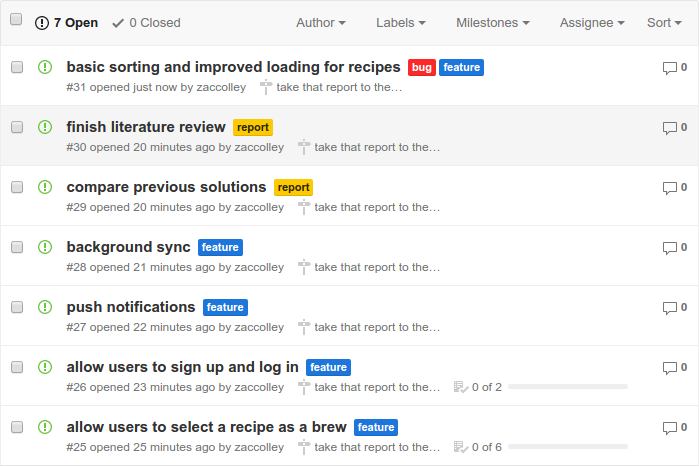
\includegraphics[width=\textwidth,height=\textheight,keepaspectratio]{github_issues}
  \caption{Example of GitHub issues setup}
  \label{figure-github-issues}
\end{figure}

\section{Requirements} \label{a-d--requirements}

Both the supervisor Rich Boakes and local Portsmouth home-brewer Alan Thompson of GetBrewing.uk, fueled the initial requirements for this project. They saw a need for applications that help improve the current home-brewing ecosystem.

As follows are requirements to create such a application to improve the brewing process when following recipes. After reviewing the current software available in section \ref{a-d--review-of-existing-software} it is clear there are problems in these areas:

\begin{itemize}
  \item Blah
  \item Blah
  \item Blah
  \item Blah
\end{itemize}

One key aspect from a lot of this software is as it is installed to a computer it is offline. Something a traditional web application couldn't achieve. Having the artefact introduce offline features makes for an innovative solution.

This application will look to solve some of these issues.

\subsection{Functional Requirements} \label{a-d--requirements--functional}

The following requirements will be structured through user stories. % cite

\subsubsection{Finding recipes}

\begin{itemize}
  \item As a \textbf{user}, I want to \textbf{search for recipes by recipe and name and description}
  \item As a \textbf{user}, I want to \textbf{browse for recipes by different recipe categories}
\end{itemize}

\subsubsection{Starting a brew}

\begin{itemize}
  \item As a \textbf{user}, I want to \textbf{select and start a brew from any recipe}
\end{itemize}

\subsubsection{Managing a brew}

\begin{itemize}
  \item As a \textbf{user}, I want to \textbf{manage the ingredients for a brew}
  \item As a \textbf{user}, I want to \textbf{be reminded at key stages of a brew}
  \item As a \textbf{user}, I want to \textbf{add notes to key stages of a brew}
  \item As a \textbf{user}, I want to \textbf{review and evaluate the brew on completion}
\end{itemize}

\subsection{Non-Functional Requirements} \label{a-d--requirements--non-functional}

The artefact should:

\begin{itemize}
  \item Follow accessibility guidelines to ensure usage for those of hard of sight
  \item Be documented so that others can maintain
  \item Conform to the performance budget that is set in initial development
  \item Pass tests generated throughout and running through continuous integration (such as Travis CI)
\end{itemize}

\section{User Interface Wireframes}

\colorbox{pink}{TODO: add wireframes}

\section{Proposed Solution} \label{a-d--proposed-solution}

Figure \ref{figure-application-stack-design}, shows an overview of the application stack to be used in the proposed solution. The following sections will describe different parts of this diagram and more.

\begin{figure}[H]
  \centering
    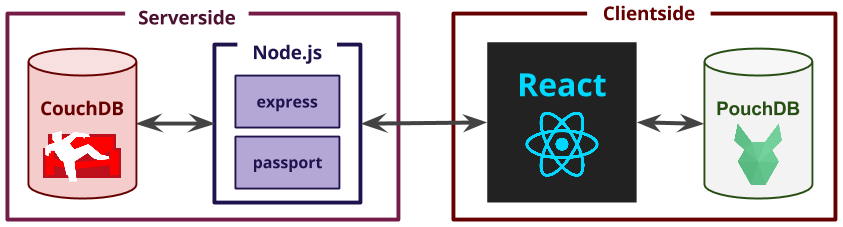
\includegraphics[width=\textwidth,height=\textheight,keepaspectratio]{application_stack_design}
  \caption{Overview of how the application stack is structured}
  \label{figure-application-stack-design}
\end{figure}

\subsection{Performance Budget}

As an initial target for the performance budget we will use a similar website speeds and try and beat them by 20\% (as explained in section \ref{l-r--performance-budgets}).

The chosen website is Malt.io, which has similar functionality to the proposed solution.

\begin{table}[H]
\centering
\begin{tabular}{|l|l|l|l|}
\hline
\textbf{Site}     & \textbf{Start Render} & \textbf{Document Complete} & \textbf{Fully Loaded} \\ \hline
Malt.to           & 2.190s                & 3.998s                     & 4.145s                \\ \hline
Proposed solution & 1.752s                & 3.1984                     & 3.316s                \\ \hline
\end{tabular}
\caption{Performance budget calculation}
\label{table-performance-budget}
\end{table}

The proposed solution will aim to have timings that are equal or below to the results in table \ref{table-performance-budget}.

With performance in mind initially the project will not implement any web fonts or images. The recipes and brew instructions have been determined as the main content and so will be the main focus.

Any iconography will use SVGs for flexibility and overall performance.

\subsection{Data} \label{a-d--data}

This sub-section will describe the gathering data and the storage of said data and creation of data.

\subsubsection{Recipe Gathering} \label{a-d--d--recipe-gathering}

As noted in section \ref{l-r--exisiting-home-brewing-solutions}, BeerXML is a popular format.
The proposed solution will scrape (process pages using scripts) existing recipe lists for BeerXML recipes.

These files will then be converted into BeerJSON which will be the main recipe format used.

\subsubsection{Databases} \label{a-d--d--databases}

Due to the format of choice BeerJSON, a document store style database that deals directly with JSON documents is a great choice.

There are many document store databases to choose from for example MongoDB, however the chosen database for the proposed solution is CouchDB for it's HTTP API and master-to-master replications. \cite{couchdb} % cite mongo

The artefact can also make use of PouchDB, a JavaScript database which leverages IndexedDB for clientside databases. PouchDB also has the same API as CouchDB allowing them to sync seamlessly.

An alternative to PouchDB would be localForage. localForage, which also allows for offline databases using IndexedDB , is faster than PouchDB however the syncing feature for PouchDB should outweigh the speed increase here. % cite speed of localforage

The proposed solution will attempt to use a Web Worker for the syncing and management of data, this will free up the main JavaScript file for presentation tasks.

\subsection{Technologies} \label{a-d--technologies}

Traditionally JavaScript has been in the browser. Node.js allows for using JavaScript on the server using Chrome's V8 JavaScript engine. \cite{node.js}

npm is a package manager for Node.js (more generally JavaScript). npm will be used for both serverside and clientside JavaScript dependencies.

The latest version of JavaScript ES2015 (also known as ES6) offers features that will be used in the proposed solution such as [....] . Support for ES2015 is mixed across browsers, therefore converting (transpiling) ES2015 to ES5 will be carried out with Babel a JavaScript transpiler. \cite{babel}

\subsubsection{Serverside} \label{a-d--t--serverside}

In this proposed solution three main packages on the serverside will be: Express, Passport and Brahaus. \cite{npm}

Express is a framework which offers features such as path routing and templating. In the proposed solution this package will be used to handle requests from the client to the server and some basic data manipulation from the database. \cite{express}

Passport is a framework for authentication, including users and user sessions. In the proposed solution this package will allow for users to sign-up, log-in and have a session in the application. \cite{passport}

Due to the artefact's knowledge base around home-brewing, a package called Brauhaus will be used. Brauhaus handles conversions of brewing recipes and brewing information. Using this package means that the home-brewing knowledge such as calculations is abstracted away, meaning developers don't necessarily to fully understand the knowledge base to create the application. \cite{brauhaus.js}

\subsubsection{Clientside} \label{a-d--t--clientside}

From the review of frameworks in section \ref{l-r--frameworks}, the proposed solution will use React as it appears to offer the best balance of features to performance.

React's usage of JSX, a syntactic sugar for improving the creation of components will be used through out the project. As SVGs will be used for graphics, JSX will complement SVG. \cite{jsx}

Using Service Workers a cache will be created to enable files to be retrieved even when offline.

\subsubsection{Styling}

For styling various technologies will be used to process into the final CSS stylesheet. CSS preprocessors convert a higher level CSS extension language with features such as variables and functions (often called mixins) to CSS.

There are many preprocessors for CSS, such as LESS, SASS or Stylus. The proposed solution will be using SASS however, due to only using the basic features being used other preprocessors could be used. \cite{SASS}

Styling often comes with some pitfalls, such as browser prefixes for CSS properties which are not stable yet. A postprocessor such as Autoprefixer. \cite{autoprefixer}

`postcss' will be used to transform these styles in the JavaScript environment. \cite{postcss}

\subsection{Workflow} \label{a-d--workflow}

As JavaScript is dynamic and loosely-typed, using a linter can ensure certain common problems are avoided. ESLint is the linter used in the proposed solution due to its extensibility and features for JSX. \cite{eslint}

Linting will be carried out with continuous integration (see section \ref{a-d--continuous-integration}) but also inside IDEs and code editors on save of JavaScript document. For this reason Atom, will be used for it's ESLint plugin.

There are many task runners for improving a development workflow such as Gulp, Grunt and Broccoli. A technology that is used in place of task runners for this artefact is Webpack. Webpack bundles all dependencies that you require and indexes them. Webpack knows what dependencies to bundle into your final file where as Gulp and Grunt have to be told which dependencies to bundle through configuration. This results in a smaller file. \cite{webpack}

A smaller file will help for the proposed performance budget and so Webpack will be used. Other technologies such as rollup, which uses `tree-shaking' to achieve a smaller bundle than Webpack can be explored but due to it's infancy this will seen as an experimental implementation. \cite{rollup}

Webpack will be used to transpile code using Babel, process Sass, process JSX from React and more.

npm will be used for clientside dependencies. Due to projects such as Browserify which create browser friendly versions of packages it is used for clientside as well as serverside JavaScript. \cite{browserify} Managers such as bower which dedicated itself to front-end dependencies has seen a drop in usage due to this. \cite{bower}

Due to the nautre of npm, dependencies depending on many different dependencies. Tracking security on dependencies is a daunting task. Snyk is a package which finds, patches and monitors vulnerabilities in your code. \cite{snyk} Snyk tests will ensure there isn't a deployed version of the build with known vulnerabilities.

With one of the non-functional requirements needing documentation, a package called commitizen will be used to enforce the contributing guidelines for project. \cite{commitizen}

\subsubsection{Continuous Integration and Deployment} \label{a-d--continuous-integration}

As ThoughtWorks describes ``Continuous Integration (CI) is a development practice that requires developers to integrate code into a shared repository several times a day. Each check-in is then verified by an automated build, allowing teams to detect problems early.". \cite{continuous_integration}

There are different ways to achieve CI, the artefact will use Travis CI. Travis CI is a online software-as-a-service CI platform. It allows developers to define a set of tasks to carry out (through a `.travis.yml` file in the repository). These tasks should have a success and fail conditions for Travis to know the status of a build. Examples of tasks include building from dependences, running tests and even miscellaneous tasks such as processing \LaTeX documents. \footnote{This report was created using \LaTeX, a word processing and document markup languages. \cite{latex} This report uses ShareLatex's CI to automatically build the final report PDF when the \LaTeX files are pushed to the GitHub repository. Magic! \cite{sharelatex}}

The deployment will also be triggered by these tests succeeding, ensuring unstable builds of the application are never deployed.

Surge (surge.sh) will being used to deploy, it is command-line tool that allows for simple deployment. Installed through npm, it removes any need for FTP, SSH or other more complicated deployment set-ups. Obviously this has limitations, but for front-end web applications this is a simple and effective option. \cite{surge}

This CI is triggered by pushing to the GitHub repository. This allows for both the code, the tests and deployment to all be together.

\section{Summary} \label{a-d--summary}

This chapter described the high-level requirements and design of a system that blah blah blah.  The chapter started by describing blah.  The proposed solution was then discussed in section blah followed by blah in section blah, etc.
Blah blah is covered in further detail in Chapter 4 which describes the implementation of blah blah.
